% !TeX program = pdflatex
% Closed-loop verification of Goldbach-related claims -- English version.
% Author list, numbers, tables and citations must stay identical to paper.tex.
\documentclass[11pt,a4paper]{article}

\usepackage[margin=2.54cm]{geometry}
\usepackage[T1]{fontenc}
\usepackage[utf8]{inputenc}
\usepackage{CJKutf8}
\usepackage{amsmath,amssymb,amsthm}
\usepackage{graphicx}
\usepackage{booktabs}
\usepackage{longtable}
\usepackage{array}
\usepackage{tabularx}
\usepackage{multirow}
\usepackage{enumitem}
\usepackage{caption}
\usepackage{xcolor}
\usepackage{url}
\usepackage[hidelinks]{hyperref}

\setlength{\emergencystretch}{3em}
\sloppy
\raggedbottom

\captionsetup{font=small,labelfont=bf,skip=6pt}
\setlist[itemize]{leftmargin=2em,itemsep=0.25em,topsep=0.35em}
\setlist[enumerate]{leftmargin=2.2em,itemsep=0.25em,topsep=0.35em}

\theoremstyle{plain}
\newtheorem{theorem}{Theorem}[section]
\newtheorem{lemma}[theorem]{Lemma}
\newtheorem{proposition}[theorem]{Proposition}
\newtheorem{corollary}[theorem]{Corollary}
\theoremstyle{definition}
\newtheorem{definition}[theorem]{Definition}
\newtheorem{remark}[theorem]{Remark}
\newtheorem{example}[theorem]{Example}

\newcommand{\BG}{\mathrm{BG}}
\newcommand{\Chen}{\mathrm{Chen}}
\newcommand{\LL}{\mathrm{LL}}
\newcommand{\WU}{\mathrm{Wu}}
\newcommand{\Even}{\operatorname{Even}}
\newcommand{\Prime}{\operatorname{prime}}
\newcommand{\PaperTheorem}{\mathrm{PaperTheorem}}
% T1 fontenc already defines \g as an accent, so the counting function is \gcount.
\newcommand{\gcount}{\mathrm{g}}
\newcommand{\N}{\mathbb{N}}
\newcommand{\R}{\mathbb{R}}
\newcommand{\Aone}{\textsf{A1}}
\newcommand{\Atwo}{\textsf{A2}}
\newcommand{\Bclass}{\textsf{B}}
\newcommand{\Cclass}{\textsf{C}}
\newcommand{\Dclass}{\textsf{D}}

\title{\bfseries Closed-Loop Verification of Goldbach-Related Claims:\\[2pt]
Textual Audit, Machine Formalization, and Independent Closure Reconstruction}
\author{\begin{CJK}{UTF8}{gbsn}宋敏、宋瑷成、宋奥菲、范钧睿、胡安、涂源\end{CJK}}
\date{17 November 2026\\[2pt]
\small Preprint v1}

\hypersetup{
  pdftitle={Closed-Loop Verification of Goldbach-Related Claims: Textual Audit, Machine Formalization, and Independent Closure Reconstruction},
  pdfauthor={宋敏, 宋瑷成, 宋奥菲, 范钧睿, 胡安, 涂源},
  pdfkeywords={Goldbach conjecture, Lean 4, formal verification, reproducibility, evidence hierarchy}
}

\begin{document}
\maketitle

\begin{abstract}
\noindent
The binary Goldbach conjecture remains open, yet weak theorems, alleged elementary proofs, and formalization artifacts are often conflated. We develop and execute a four-stage closed-loop protocol: claim decomposition with version pinning, line-level textual audit, reproducible finite computation, Lean~4 formalization with axiom audit, and manifest-constrained independent reconstruction of an import closure. Evidence is classified as A1 (kernel theorem), A2 (artifact pass), B (textual fact), C (finite computation), or D (judgment). Three linked cases yield different verdicts. First, under its own definition of big-$\mathcal O$ (ratio tending to a nonzero constant), the statement of Theorem~1.1 in arXiv:2611.09007v1 already implies binary Goldbach; its proof lists the current case $G(2n)$ among the assumptions, making the argument circular; it also takes the positivity of $G(2n-2)$ as an input, which under the literal definition already presupposes the positivity required by the conclusion and under the standard reading lacks a basis; equations (1)--(2) are each off by one in opposite directions for every $3\le x\le 6000$. Neither the literal nor the standard-$\mathcal O$ reading supports the proof claim. Second, eight Lean~4 theorems show that binary Goldbach implies Chen $1+2$, Li--Liu $1+1.9$, and Wu $1+1.8938$; the endpoint predicates are strictly wider, but this is neither an independence proof nor a converse. Third, we independently rebuild the 3,764-module import closure of the Wu endpoint: zero real failures, 3,764/3,764 source hashes matching the manifest (30,215,769 bytes; 621,451 physical lines), six endpoint declarations depending exactly on the three standard axioms, and a successful \texttt{leanchecker} replay of the endpoint module. The reconstruction is artifact-level, not clean-room, and does not verify the prose of the Wu paper. We conclude that Goldbach remains open and that the value of closed-loop verification lies in separating proof claims, formal artifacts, finite evidence, and residual uncertainty.

\vspace{0.6em}
\noindent\textbf{Keywords:} Goldbach conjecture; formal verification; Lean~4; reproducibility; evidence hierarchy; mathematical audit

\vspace{0.3em}
\noindent\textbf{MSC 2020:} 11P32 (Goldbach problem); 68V20 (Formalization of mathematics); 03B35 (Proof assistants)
\end{abstract}

\vspace{0.4em}
\noindent\rule{\textwidth}{0.4pt}
\begin{flushleft}
\small
\textbf{Version and scope.} This is a preprint, not a proof of the Goldbach conjecture. Every occurrence of ``verified'' or ``rebuilt'' below carries an explicit scope; all formal conclusions concern only the Lean statements listed, and all numerical conclusions concern only the finite ranges listed. See the data-and-code availability section for how to obtain the code, hashes and logs.
\end{flushleft}
\noindent\rule{\textwidth}{0.4pt}

\newpage
\section{Introduction}
\label{sec:intro}

In 1742 Goldbach wrote to Euler that every even integer greater than $2$ is a sum of two primes. That statement---today the binary (strong) Goldbach conjecture---remains open. Twentieth-century analytic number theory produced a chain of weaker results: Chen's $1+2$ theorem writes a large even integer as ``a prime plus a number with at most two prime factors''\cite{chen1973,chen1978}; the Li--Liu $1+1.9$ theorem writes a large even integer as $p+rq$ with $r=1$ or $r$ prime and $r^{10}\le q^{9}$\cite{liliu}; Wu's $1+1.8938$ endpoint has the same shape with the exponent condition strengthened to $r^{5000}\le q^{4469}$\cite{upstream}. These results are commonly summarised in the press as ``a hair's breadth from $1+1$'', but the logical direction is the opposite: $1+1$ \emph{implies} these endpoints (take $r=1$), whereas the endpoints are not known to imply $1+1$. Describing a weak result as ``nearly finished'' is one of the most common category errors in public understanding.

In November 2026 a nine-page preprint appeared on arXiv, titled \emph{An Elementary Proof of the Binary Goldbach Conjecture}\cite{qazaqzeh}. At the same time the public Lean~4 project \texttt{goldbach-lean} had already formalized the Chen, Li--Liu and Wu routes and, in its research sub-project, a formal statement of the Wu endpoint\cite{upstream}. Three lines---paper proof, numerical experiment, machine formalization---arrived in the same period, which makes a methodological question urgent: \emph{given a ``proof'', a ``formalization'' and an artifact that ``compiles'', what can we actually conclude about each?}

``The Lean build passes'' is not ``the paper's mathematical argument is correct''; ``the source hashes match'' is not ``the theorem statement is faithful to the paper''; ``verified up to $4\times 10^{18}$'' is not ``true for all even integers''; and ``the endpoint passes the kernel'' is not ``the Goldbach conjecture is proved''. These distinctions are well known in principle, yet in concrete work they are easily flattened by a binary \texttt{PASS}. This is especially so once generative AI can mass-produce text, code and formalization scripts that look rigorous: the bottleneck is no longer whether a proof can be written, but whether a claim can be judged, in the right scope and at the right evidence level, for what it actually establishes.

We treat this as a \emph{closed-loop verification} problem: starting from the original claim, four stages---text, numerics, formalization and independent reconstruction---each answer a different question, produce a different evidence level, and explicitly return whatever did not close to the next round. We propose no new logical system and prove no new number-theoretic theorem; we propose and test a reusable audit protocol, and use three cases to show how it behaves when falsifying a proof claim, formalizing an endpoint hierarchy, and independently rebuilding a large closure.

\subsection{Research questions}
\label{sec:rq}

We organise the paper around four questions.

\begin{itemize}
\item \textbf{RQ1 (text level)} Given a specific proof text, can one locate definition substitution, circular assumptions, a missing base case, and uncontrolled error terms without relying on the author's intent, and back each finding with line-level evidence?
\item \textbf{RQ2 (formal level)} Can the key ``direction facts'' and ``circularity interface'' be formalized as a minimal Lean module that depends only on the standard axioms and can be replayed independently?
\item \textbf{RQ3 (reconstruction level)} For a large formalization closure, can one rebuild it independently under fixed sources, a fixed toolchain and a fixed manifest, and state precisely what ``the build passes'' covers and what residual risk remains?
\item \textbf{RQ4 (method level)} How should this evidence be graded so that finite computations are not upgraded to universal conclusions, artifact passes to mathematical theorems, and formal statements to the paper's intent?
\end{itemize}

\subsection{Contributions}
\label{sec:contributions}

The contributions can be summarised in five points.

\begin{enumerate}
\item \textbf{A four-stage closed-loop protocol.} Claim decomposition, textual audit, numerical recomputation, formalization and closure reconstruction are organised into a feedback loop, with inputs, outputs, stop conditions and hard boundaries specified for each stage (Section~\ref{sec:framework}).
\item \textbf{An operational evidence grading.} The labels A1/A2/B/C/D distinguish kernel theorems, artifact passes, textual facts, finite computations and judgments, together with the rule that nothing may be upgraded across levels (Section~\ref{sec:framework}, Table~\ref{tab:evidence}).
\item \textbf{A concrete falsification case.} For arXiv:2611.09007v1 we exhibit the dilemma between the literal and the standard reading: the former makes Theorem~1.1 imply $1+1$ and exposes the circularity, the latter deprives the key positivity step of its basis; we also give pointwise counterexamples to equations (1)--(2) (Section~\ref{sec:paper}).
\item \textbf{A set of kernel-checked direction theorems.} Eight Lean~4 theorems turn ``$1+1\Rightarrow$ the three endpoints'' and ``the paper's theorem under its own $\mathcal O$ definition $\Rightarrow 1+1$'' into replayable propositions, with three witnesses that the representation predicates are strictly wider (Section~\ref{sec:endpoints}).
\item \textbf{A large independent reconstruction.} The 3,764-module import closure of the Wu endpoint is rebuilt locally, reporting zero real failures, matching source hashes, the standard axioms and the endpoint replay, while stating explicitly that it is neither clean-room, nor research-wide, nor a verification of the paper (Section~\ref{sec:wu}).
\end{enumerate}

The fifth contribution needs qualification in particular: what it confirms is that a \emph{formal artifact} compiles under this toolchain and that the endpoint declarations pass the kernel, not that Wu's paper proof is mathematically correct, and certainly not the Goldbach conjecture itself. Section~\ref{sec:wu} lists sentence by sentence what may and may not be written.

\subsection{Organisation}
\label{sec:organization}

Section~\ref{sec:background} recalls the weak Goldbach results, the Lean trust chain and related work. Section~\ref{sec:framework} describes the protocol, the evidence levels and the decision rules. Sections~\ref{sec:paper}, \ref{sec:endpoints} and \ref{sec:wu} treat the preprint, the endpoint hierarchy and the Wu closure. Section~\ref{sec:synthesis} assembles the claim matrix, discusses the limits of closed loops and reflects on the originality of this work. Section~\ref{sec:threats} discusses threats to validity and Section~\ref{sec:conclusion} concludes. The appendices list the Lean declarations, the reproduction commands and the evidence inventory.

\section{Background and related work}
\label{sec:background}

\subsection{The Goldbach conjecture and weak approximations}
\label{sec:bg}

We use the following formal statement. The proposition $\BG$ holds if there is $N_0$ such that every even $N\ge N_0$ is a sum of two primes:
\begin{equation}
\BG:\quad \exists N_0\in\N,\ \forall N\ge N_0,\ \Even(N)\Longrightarrow
\exists p,q\in\N,\ p\ \text{prime}\land q\ \text{prime}\land N=p+q.
\label{eq:bg}
\end{equation}
``Sufficiently large'' is an existential quantifier, not an assertion about all $N$; this must be preserved in formalization, or ``large even integers'' silently becomes ``all even integers''.

The three weak endpoints are defined as follows. Chen's $1+2$ allows the second summand to be a prime or a product of two primes:
\begin{equation}
\begin{aligned}
\Chen:\quad &\exists N_0,\ \forall N\ge N_0,\ \Even(N)\Longrightarrow
\exists p,q\in\N,\ p\ \text{prime}\ \land\\
&\bigl(q\ \text{prime}\ \lor\ \exists r,s\in\N,\ r,s\ \text{prime}\land q=rs\bigr)
\land N=p+q.
\end{aligned}
\label{eq:chen}
\end{equation}
Li--Liu $1+1.9$ and Wu $1+1.8938$ share one shape
\begin{equation}
\exists T,\ \forall N\ge T,\ \Even(N)\Longrightarrow
\exists p,r,q\in\N,\ p,q\ \text{prime}\land (r=1\lor r\ \text{prime})
\land N=p+rq\land r^{a}\le q^{b},
\label{eq:family}
\end{equation}
with $(a,b,T)=(10,9,4)$ for Li--Liu and $(a,b,T)=(5000,4469,512)$ for Wu\cite{liliu,upstream}. Since $4469/5000=0.8938<0.9=9/10$, Wu's condition is stronger than Li--Liu's; and since $rq$ has at most two prime factors when $r=1$ or $r$ is prime, Wu's endpoint implies Li--Liu's, which implies Chen's. This direction is one of the facts machine-checked in Section~\ref{sec:endpoints}.

The weak (ternary) Goldbach conjecture---every sufficiently large odd integer is a sum of three primes---was proved by Helfgott\cite{helfgott}; it is a different problem from the binary conjecture and cannot replace it. The notation needs emphasis. $1+2$ is not ``$1$ plus $2$'', and $1+1.9$ is not ``$90\%$ done''. $1+a$ says the second summand has at most two prime factors, with the size ratio controlled by $r\le q^{a-1}$. The closer $a$ is to $1$, the stronger the condition; but even at $a=1.8938$, $r$ may still be prime, so this is not $1+1$. The obstacle from $1+2$ to $1+1$ is not ``compute a little further'' but the parity problem of sieve theory: the Selberg sieve detects ``not divisible by small primes'' and cannot distinguish an even number of prime factors from an odd one, so it cannot force the second summand to have exactly one prime factor\cite{montgomery-vaughan}. This is the key to understanding why a weak result is not half a proof.

Finite verification is a different kind of evidence. Oliveira e Silva, Herzog and Pardi verified by computation all even integers up to $4\times10^{18}$\cite{oliveira2014}; a 2026 preprint reports a window of length $10^{15}$ beyond $4\times10^{18}$, explicitly conditional on that earlier verification\cite{llorente2026}. These are important empirical facts, but they are finite statements $\forall N\le X$, not the infinite statement $\forall N$. We grade them as C-level evidence and do not upgrade them because the range is large.

\subsection{Lean~4, the kernel and the trust chain}
\label{sec:lean}

Lean~4 is a proof assistant based on dependent type theory whose trusted kernel checks whether a term has the claimed type\cite{lean4}. Mathlib provides a large mathematics library\cite{mathlib}. Ideally, a Lean declaration
\begin{center}
\texttt{theorem t : P := ...}
\end{center}
passing the kernel means $P$ is provable under the axioms and definitions used. Users can inspect the axioms a declaration depends on with \texttt{\#print axioms t}; we accept only axiom sets contained in
\[
\{\texttt{propext},\ \texttt{Classical.choice},\ \texttt{Quot.sound}\},
\]
and separately scan for \texttt{sorry}, \texttt{admit}, user-defined \texttt{axiom}, \texttt{native\_decide}, \texttt{unsafe} and \texttt{skipKernelTC}. These checks are the practical version of de Bruijn's criterion: correctness must be guaranteed by a small, auditable checker, not by the prover's or the generating model's self-report\cite{geuvers2009}.

Formalization has a further trust chain that is often ignored: \emph{the transcription of the statement}. The kernel checks ``this term has this type''; it does not check ``this type is faithful to the paper's proposition''. If a formal statement renders ``sufficiently large'' as ``all'', a ``nonzero limit'' as an ``upper bound'', or ``at most two prime factors'' as ``two primes'', the kernel will happily accept a theorem different from the intended one. Avigad summarizes this as the semantic distance between formalization and mathematical practice\cite{avigad2018}. We therefore place statement audit before formalization and restrict the scope of A1 strictly to ``the formal statements listed'', never to ``the paper's intent''.

A further common misunderstanding concerns \texttt{leanchecker}. In Lean~4.33, \texttt{leanchecker} replays only the proof terms \emph{newly declared} by the target module on top of its import environment; it is not a second independent kernel and does not replay all imported modules. Its own source states, in essence, that it is a tool for detecting environment tampering rather than an external verifier. When reporting the Wu endpoint replay we therefore write ``only the module \texttt{WR2ClassicalCertificate} is replayed'', and never ``all 3,764 modules are replayed''.

\subsection{Related work}
\label{sec:related}

Machine formalization of large mathematical proofs has mature precedents. Gonthier's formal proof of the four-colour theorem\cite{gonthier2008} and Hales et al.'s Flyspeck project\cite{hales2017} show that formalization can independently check computations and classifications that are hard to verify by hand. Scholze's liquid tensor experiment demonstrated its role in clarifying definitions and proof dependencies in modern mathematics\cite{scholze2022}. Together these establish that the value of formalization is not only error prevention but making implicit definitions, quantifiers and dependencies explicit.

On reproducibility, Peng distinguishes repeatability, reproducibility and recomputability\cite{peng2011}; Donoho et al. discuss binding results, code and data in computational science\cite{donoho2009}. Our closure reconstruction borrows from this tradition but changes the object to ``source manifest + fixed toolchain + kernel artifact'': not only must the command re-run, it must run on sources byte-identical to the manifest, and failure semantics must be fail-closed.

The closest work to ours is the upstream \texttt{goldbach-lean} project itself\cite{upstream}, which formalized the Chen and Li--Liu routes and collected Wu's sources and acceptance records under \texttt{research/wu2008/}. We do not redo its mathematical development; we build three things on top of it: a replayable theorem that the endpoints are weaker than $1+1$; a formalization of one preprint's $\mathcal O$ definition and circularity interface; and one independent, scope-limited rebuild of the Wu endpoint's import closure. Within our limited November 2026 search we found no public combination of these three; we performed no exhaustive search and therefore claim no priority.

\section{The closed-loop verification framework}
\label{sec:framework}

\subsection{Design principles}
\label{sec:principles}

We use a multi-case, artifact-centred design. The three cases are not a random sample; they are critical cases chosen by evidence type: case one tests the text, definition and numerical layers, case two the formalization layer, case three the large-scale build layer. Four selection criteria applied: (i) the audited object has a publicly checkable version and hash; (ii) a replayable Lean interface or source manifest exists; (iii) the verdict types differ (refutation, formal support, artifact pass) and cover the main branches of the decision matrix; (iv) the boundaries of failure and success can be written as checkable sentences. Case studies do not aim at statistical representativeness but at whether the framework yields an auditable verdict in the critical situations.

The framework rests on five principles.

\begin{enumerate}
\item \textbf{Claim relativity.} There is no ``verified'' independent of a specific claim. The same artifact may support ``this Lean code passes the kernel'' but not ``this paper proves the conjecture''. A verification report must render the claim as a decidable sentence and bind evidence item by item.
\item \textbf{Explicit scope.} Every conclusion must state its quantifier scope (all $N$ / $N\le X$ / this version / this import closure), its toolchain version and its source hashes. Scope is not a footnote but part of the conclusion.
\item \textbf{No upward conversion.} A finite computation may not be upgraded to a universal theorem; an artifact pass may not become a mathematical proof; a textual fact may not become a refutation of the author's entire work; a formal theorem may not automatically become a faithful transcription of the paper's intent.
\item \textbf{Adversarial stance.} Seek evidence that could overturn the claim first: counterexamples, circularity, missing base cases, uncontrolled error terms, hash mismatches, missing artifacts. A process that only collects supporting evidence is endorsement, not verification.
\item \textbf{Version pinning.} Hash the audited text, sources, dependencies and toolchain; every line reference binds to a version. If the version changes, earlier conclusions are marked ``for v1'' and are not inherited automatically.
\end{enumerate}

\subsection{The four stages}
\label{sec:stages}

Figure~\ref{fig:pipeline} gives an overview. Stage S0 decomposes the claim, and S1--S4 correspond to text, numerics, formalization and reconstruction. Every stage can send work back upstream: a textual audit that finds an unclear definition changes the formal statement; a formalization that cannot transcribe the statement faithfully demands another textual audit; a reconstruction whose sources disagree with the manifest aborts and returns to version pinning.

\begin{figure}[htbp]
\centering
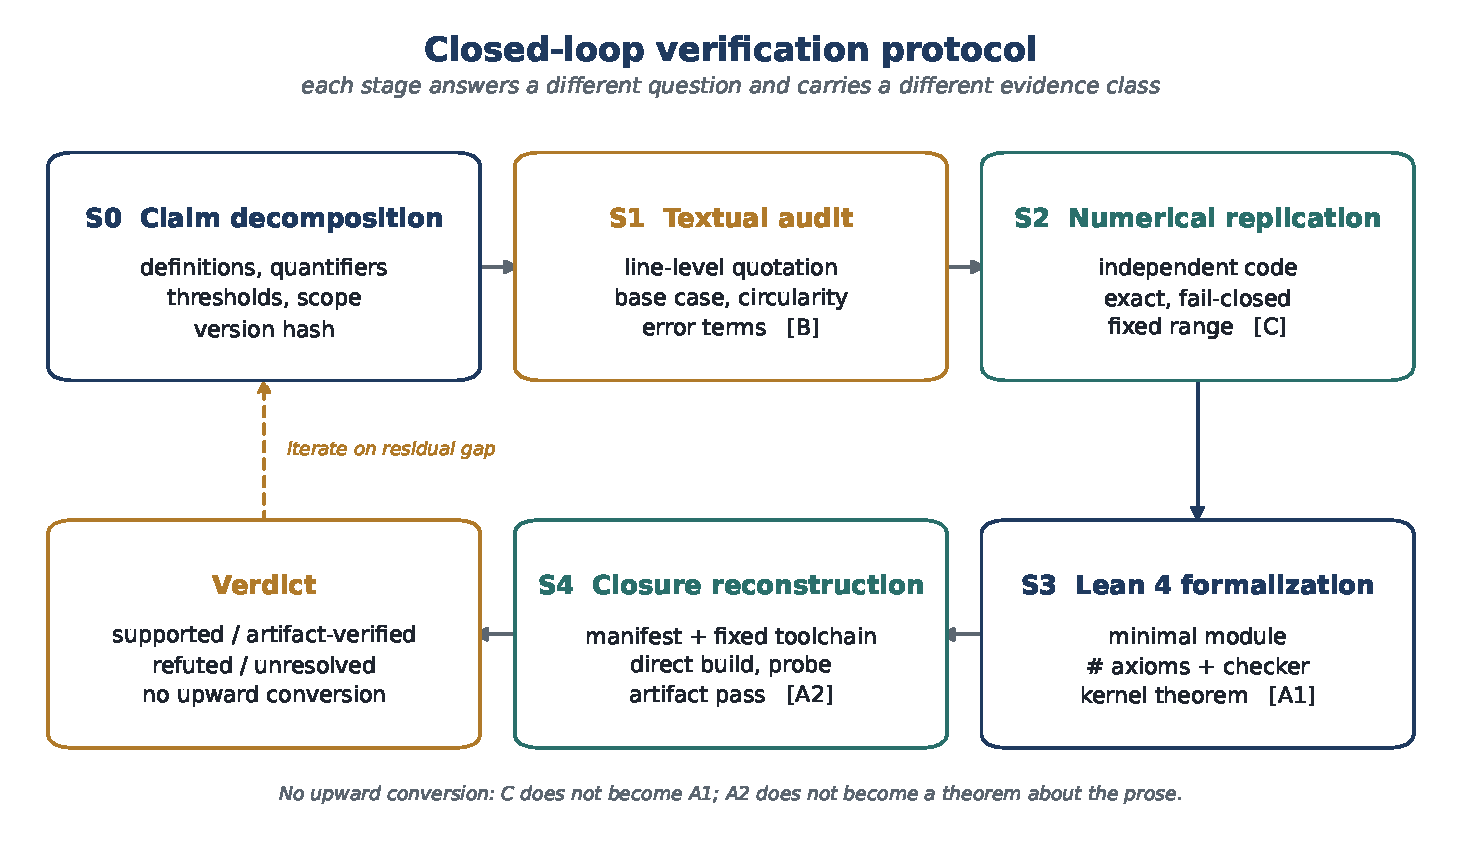
\includegraphics[width=\textwidth]{figures/fig1_pipeline.pdf}
\caption{The four-stage closed-loop protocol. Each stage answers a different question and yields a different evidence level; residual semantic or scope gaps are sent back to S0/S1 rather than hidden by a pass.}
\label{fig:pipeline}
\end{figure}

\paragraph{S0: claim decomposition and version pinning.}
Split the original claim into definitions, quantifiers, thresholds, dependencies and scope. Compute a SHA-256 of the text, a manifest hash of the sources, and record toolchain versions. The resulting claim graph must answer: which definitions does this claim depend on? On which line of the original do they appear? Is the threshold ``exists'' or ``for all''? Does the conclusion cover the whole text, a section, or one formal statement?

\paragraph{S1: line-level textual audit.}
Anchored on line numbers, check definitional consistency, quantifier direction, base cases, circular assumptions, limits and error terms, constant consistency, and omitted steps such as ``obviously'' and ``similarly''. Output B-level textual facts: each must be ``the original line $n$ plus a logical analysis'', never ``I think this is wrong''. For critical passages keep the English original and give a translation, so that paraphrase does not distort.

\paragraph{S2: reproducible numerical checks.}
Recompute identities, counts and numerical assertions with independent code. Requirements: fixed range, exact arithmetic (or an explicit error bound), fail-closed semantics, and scripts saved together with results. A numerical check cannot prove a universal statement, but it can refute a universal numerical assertion; it can also expose empirical signals such as ``the data do not support this constant limit''. Output C-level evidence.

\paragraph{S3: Lean~4 formalization and axiom audit.}
Formalize only the \emph{critical interface}, not the whole paper. The critical interface is usually one contested definition, one directional implication, one circular step, or one bridge connecting positivity with representation. Keep the module small and depend only on the necessary libraries; print the axiom set with \texttt{\#print axioms}, replay the target module with \texttt{leanchecker}, and exclude forbidden tokens by static scan. Output A1-level evidence, whose scope is strictly the formal statement.

\paragraph{S4: independent closure reconstruction.}
With sources, dependency manifest and toolchain fixed, bypass the original build scheduler and invoke the compiler directly to rebuild the import closure of the target endpoint. Requirements: record each module's exit code; count a module as complete only when both an \texttt{.olean} and a success marker exist; stop on failure with a resumable state; the final audit checks source hashes, forbidden tokens and artifact completeness together. Output A2-level evidence: it states that ``this source set is accepted by the kernel under this toolchain'', not that ``the paper's mathematical argument is correct''.

\subsection{Evidence levels and decision rules}
\label{sec:evidence}

Table~\ref{tab:evidence} lists the five evidence classes. A1 and A2 both involve the kernel but concern different objects: A1 is ``the proof term of a formal statement passes the check'', A2 is ``a source closure compiles and the endpoint probes pass''. B is a textual fact, C a finite computation, D a judgment. The classes are not honour levels but marks of \emph{applicability}: A1 is not ``truer'' than B, it answers a different question.

\begin{table}[htbp]
\centering
\small
\caption{Evidence levels: what each level can and cannot support}
\label{tab:evidence}
\begin{tabularx}{\textwidth}{@{}>{\raggedright\arraybackslash}p{0.10\textwidth}
>{\raggedright\arraybackslash}p{0.27\textwidth}
>{\raggedright\arraybackslash}X
>{\raggedright\arraybackslash}p{0.24\textwidth}@{}}
\toprule
Level & Criterion & Can support & Cannot support\\
\midrule
\Aone & Lean declaration passes the kernel; \texttt{\#print axioms} and \texttt{leanchecker} records complete & The listed formal statement holds under the given axioms and definitions & The paper's intent, mathematical importance, steps not formalized\\
\addlinespace
\Atwo & Source hashes match the manifest; build completes under the fixed toolchain; endpoint probes pass & This source closure is accepted by the kernel under this toolchain & The paper's prose, clean-room reconstruction, the whole research scope\\
\addlinespace
\Bclass & Line-addressable citation plus analysis of definitions, quantifiers and circularity & Specific textual defects, definitional inconsistency, circular interfaces & Refutation of the author's entire work, other versions\\
\addlinespace
\Cclass & Reproducible script plus fixed finite range plus exact arithmetic or error bounds & The finite proposition on the listed range & Universal statements, extrapolation beyond the range\\
\addlinespace
\Dclass & Expert judgment, research taste, directional opinion & Hypotheses, conjectures, next steps & Factual conclusions\\
\bottomrule
\end{tabularx}
\end{table}

Verdicts are four-valued rather than binary:
\begin{itemize}
\item \textbf{supported} the claim is semantically consistent with the formal statement, and A1/A2 evidence covers all critical parts of the claim.
\item \textbf{artifact-verified} the artifact passes the checks, but the semantic or scope layer of the claim is not closed; a ``limited to \ldots'' qualifier is mandatory.
\item \textbf{refuted} a necessary step of the claim is overturned by a concrete counterexample, a circularity, or a definitional contradiction; the refutation concerns only the listed version and the listed claim.
\item \textbf{unresolved} the available evidence neither supports nor refutes the claim; unresolved is neither ``true by default'' nor ``false by default''.
\end{itemize}

The most important rule is ``no upward conversion'': C does not become A1 because the range is large; A2 does not become a theorem about the paper because ``the kernel passed''; B does not become a universal conclusion because ``the author did not respond''. Conversely, A1 must not be dismissed as ``mere formalization'': it is exactly what pins down the directionality and the circularity interface and gives the dispute an inspectable object.

\subsection{Stop conditions and completeness gates}
\label{sec:stops}

A stage may stop only when the following conditions hold:

\begin{itemize}
\item \textbf{Text stage:} the critical definitions, quantifiers, base cases, circular interfaces and error terms are located; every judgment carries a line number; the version of the audited text is hashed.
\item \textbf{Numerics stage:} the script runs independently; range and failure semantics are stated; results are compared item by item with the assertions in the text; counterexamples are recomputable.
\item \textbf{Formal stage:} the module compiles; the axiom set is a subset of the three standard axioms; no forbidden tokens; \texttt{leanchecker} replays the target module; the correspondence between formal statements and textual definitions is written out item by item.
\item \textbf{Reconstruction stage:} source hashes match the manifest; every target module has its artifacts; the forbidden-token scan is zero; the endpoint probes pass; the final status file folds source identity, lexis and artifact completeness into its verdict.
\end{itemize}

Completeness gates are not formalism. An early version of our Wu reconstruction still printed \texttt{PASS} while 690 build artifacts were missing, because \texttt{missing\_build\_artifact} was written only into the JSON and never entered the final status. After the fix, the status requires source identity, lexis and artifact completeness simultaneously. The example shows that the meaning of a \texttt{PASS} depends on its decision function; leaving completeness out of that function misreads ``the sources are right'' as ``the build is complete''.

\subsection{What the framework does not do}
\label{sec:not-do}

The framework does not replace peer review, does not prove mathematical conjectures, does not judge research taste, and does not deliver a verdict on the author's honesty. It does one thing: it splits a composite claim into separately checkable parts and records the applicability of the evidence for each. For the preprint discussed here we evaluate only its text and the steps listed, not the author's other work; for the upstream formalization project we evaluate only the closure we rebuilt, not all of its 4,151 modules; for the Goldbach conjecture itself we claim no new proof.

\section{Case one: the definitions and circularity of an ``elementary proof''}
\label{sec:paper}

\subsection{Object and version}
\label{sec:paper-object}

The audited object is the preprint \emph{An Elementary Proof of the Binary Goldbach Conjecture} by Khaled Qazaqzeh and Aymen Rawashdeh, arXiv:2611.09007v1, 6 November 2026, math.NT, 9 pages\cite{qazaqzeh}. All line numbers below refer to the LaTeX source of v1, \texttt{A\_Simple\_Proof\_of\_Goldbach\_Conjecture.tex}, not to PDF page numbers. The SHA-256 of that source is
\begin{center}
\texttt{db1fa07154ae7430245d19ac377f6d22f\\02361608014498fe3449129c3765ffd},
\end{center}
and the local copy is byte-identical to the source offered with arXiv v1 (checked 15 November 2026). The hash pins the version, so readers can re-check the line numbers independently of this paper.

We evaluate only the preprint's proof claim, not the authors' other work, and we do not claim that ``every step of the paper is wrong''. On the contrary, we point out below some correct observations (for example the symmetry $H=K$; $G,H,D,K$ are the four counting functions defined in Section~2 of the paper, and we do not repeat their definitions), which marks the boundary of the audit.

\subsection{Definition: a non-standard $\mathcal O$}
\label{sec:paper-def}

The first clause of Definition~2.1 (source line 111) reads:

\begin{quote}\itshape
``We say that $f$ is a big $\mathcal O$ of $g$, denoted by $\mathcal O(g)$, if
$\lim_{n\to\infty} f(n)/g(n)=c$ for some nonzero real number $c$.''
\end{quote}

\noindent That is: $f$ is a big $\mathcal O$ of $g$ if $f(n)/g(n)\to c$ for some nonzero real $c$.

The standard big $\mathcal O$ only requires a constant $C$ with $|f(n)|\le C g(n)$ eventually; it allows the ratio to be $0$ or not to exist. The preprint's definition requires the ratio to \emph{converge to a nonzero constant}, a far stronger two-sided asymptotic condition. Under that definition, ``$G(2n)=\mathcal O(n/\ln^2 n)$'' means
\begin{equation}
\lim_{n\to\infty}\frac{G(2n)\ln^2(2n)}{n}=c\ne0.
\label{eq:paperO}
\end{equation}
where $G(2n)$ is the (ordered) number of Goldbach representations of $2n$. Theorem~1.1 states $\ln^2 n$, whereas lines 182/184 of the proof use $\ln^2(2n)$; since $(\ln(2n)/\ln n)^2\to1$, the nonzero limit is unaffected. Our formalization uses the $\ln^2(2n)$ form that appears in the proof.

\subsection{The dilemma: literal versus standard reading}
\label{sec:dilemma}

There are two readings of the definition on line 111. Neither supports the paper's proof claim.

\paragraph{Reading A (literal).}
Taking line 111 strictly, Theorem~1.1 is not an ``upper bound'' but an asymptotic lower bound with a nonzero constant. From $G(2n)\ge0$ we get $c\ge0$; from $c\ne0$ we get $c>0$; hence $G(2n)>0$ eventually, i.e.\ every sufficiently large even integer is a sum of two primes. That is, \emph{under this definition Theorem~1.1 already implies $1+1$}. This does not say that Theorem~1.1 has been proved, only that its statement already contains the conclusion; if the proof then assumes that conclusion, the argument is circular. The next subsection gives the formal theorem and Section~\ref{sec:circularity} the line-level evidence.

\paragraph{Reading B (standard).}
If the authors intended the standard big $\mathcal O$ (an upper bound only), Theorem~1.1 no longer implies $G(2n)>0$; a counting function that vanishes identically satisfies the upper bound. Then the steps deriving ``$G(2n-2)>0$'' or ``$\alpha<2$'' from ``$G(2n-2)=\mathcal O(n/\ln^2 n)$'' lose their basis, and the paper offers no alternative positivity argument. So under the standard reading the proof fails as well; only the location of the failure moves from ``circularity'' to ``missing positivity step''.

\paragraph{Conclusion.}
Under both readings the paper fails to establish that every large even integer is a sum of two primes. The literal reading exposes self-containment at the statement level and circularity at the proof level; the standard reading exposes a missing key estimate. The dilemma is stronger than pointing out that ``the $\mathcal O$ definition is non-standard'': it shows that the problem lies not in a symbol's usage but in the logical interface between theorem, proof and conclusion.

\subsection{Formalization: Theorem~1.1 implies $1+1$}
\label{sec:paper-formal}

Let
\begin{equation}
\gcount(N):=\#\{p\le N:\ p\ \text{prime}\land N-p\ \text{prime}\}.
\label{eq:count}
\end{equation}
$\gcount$ counts each admissible $p$ once, hence counts ordered representations (the diagonal case once). For $N\ge6$, $p=2$ contributes nothing because $N-2$ is an even integer larger than $2$ and therefore composite; on the relevant range $\gcount(2n)$ thus agrees with the paper's $G(2n)$. We formalize the content of Theorem~1.1 under its own $\mathcal O$ definition as
\begin{equation}
\PaperTheorem:\quad \exists c\in\R,\ c\ne0,\quad
\lim_{n\to\infty}\frac{\gcount(2n)\ln^2(2n)}{n}=c.
\label{eq:papertheorem}
\end{equation}

\begin{theorem}[self-containment of the paper's theorem]
\label{thm:paper-implies-bg}
$\PaperTheorem\Longrightarrow\BG$.
\end{theorem}

\begin{proof}
Let $a_n:=\gcount(2n)\ln^2(2n)/n$. By $\PaperTheorem$, $a_n\to c\ne0$.

\begin{enumerate}[label=(\roman*)]
\item Since $\gcount(2n)\ge0$, $\ln^2(2n)\ge0$ and $n>0$, eventually $a_n\ge0$, hence $c\ge0$.
\item Since $c\ne0$, we get $c>0$.
\item Since $a_n\to c>0$, eventually $a_n>0$. For those $n$, $\ln^2(2n)>0$ and $n>0$, so $\gcount(2n)>0$.
\item $\gcount(2n)>0$ means there are primes $p,q$ with $2n=p+q$. Hence every sufficiently large even integer is a sum of two primes, i.e.\ $\BG$.
\end{enumerate}
\end{proof}

In Lean~4 the theorem is called \texttt{paperTheorem\_implies\_binaryGoldbach} and sits in \texttt{Goldbach/Gap.lean} with the other seven theorems, its axiom set being the three standard axioms; Section~\ref{sec:endpoints} gives the full verification record. The theorem states only that ``under the literal definition, Theorem~1.1 implies $1+1$''; it does not state that ``the paper proves Theorem~1.1'', still less that ``the Goldbach conjecture is proved''. It moves the dispute from ``is the $\mathcal O$ written wrongly'' to ``does the proof really establish this statement''.

\subsection{Where the circularity is}
\label{sec:circularity}

A strong theorem statement is not yet a circular proof; the circularity is at the start of the proof. Line 180 of the preprint's source reads (emphasis added; cross-references rendered as numbers):

\begin{quote}\itshape
``We proceed by induction on $n$ to verify the claim of the theorem. Thus we can assume that
$G(2n-2)$ \textbf{and} $G(2n)$ are $\mathcal O\bigl(n/\ln^{2} n\bigr)$ functions as a
consequence of the result of Lemma (note). As a consequence of Equation (1), the induction
hypothesis on the antidiagonals $I_{2n-2}$, \textbf{the positivity of $G(2n-2)$} and the
result of Lemma (note), we conclude \ldots''
\end{quote}

\noindent Read literally, this passage puts $G(2n)$---the very case to be proved---among the objects that may be assumed. An induction hypothesis should supply only the case $n-1$, namely $G(2n-2)$; deriving $G(2n)$ from $G(2n-2)$ needs an independent recursion, which the paper does not give. The same sentence also lists $G(2n-2)>0$ as an input. We treat this separately and do not merge it into the circularity verdict: under the literal definition, ``$G(2n-2)=\mathcal O(n/\ln^2 n)$'' already implies $G(2n-2)>0$ eventually, so it already presupposes the positivity required by the conclusion (B); under the standard reading, the positivity step loses its basis. Line 184 then derives $\alpha<2$ from the same $\mathcal O$ statement; if $G(2n-2)\sim c\,n/\ln^2 n$ then $\alpha=2-c$, and $\alpha<2$ is equivalent to $c>0$, again the same positivity.

The circularity therefore has two precise formulations; a separate positivity-reading issue is not part of the circularity verdict:

\begin{itemize}
\item \textbf{The machine-checked part:} under the literal $\mathcal O$ definition, Theorem~1.1 implies $\BG$ (Theorem~\ref{thm:paper-implies-bg}).
\item \textbf{The text-comparison part:} line 180 literally lists $G(2n)$ itself among the assumptions; this is the circularity evidence, and on this point the induction step assumes the current case to be proved.
\item \textbf{The separate positivity-reading part:} the same sentence takes $G(2n-2)>0$ as an input; under the literal definition this already presupposes the positivity required by the conclusion (B), while under the standard reading it lacks a basis. This item is not circularity evidence.
\end{itemize}

These two pieces of evidence have different levels (A1 and B) and must not be conflated. We do not say ``Lean proved that the paper is circular''; Lean proves a conditional implication, while the circularity verdict comes from reading line 180 word by word. Keeping the two apart is a concrete application of the evidence grading in this paper.

\subsection{Other textual and numerical problems}
\label{sec:paper-other}

Beyond the circularity, the audit found the following problems. They are not evidence that ``the whole paper is wrong'', but each independently weakens its reliability.

\paragraph{No base case.}
The inductive argument provides no starting point. Even if every recursion step held, at least one $n_0$ with $G(2n_0)>0$ is needed, and the paper does not supply it explicitly. For a ``sufficiently large'' statement such as Goldbach, the base case could be covered by finite verification, but the paper neither cites nor constructs one.

\paragraph{The $R_1$ assertion is not controlled by the induction hypothesis.}
Around line 222 the paper says that, by the induction hypothesis, one may assume $R_1=o(n/\ln^2 n)$. But $R_1$ counts four-point configurations (tuples involving ``three primes plus one composite''), which is not the same object as the $G$ count; a bound on $G$ cannot control $R_1$. The sentence is not a derivation but a renaming of the hardest estimate, then an assumption. Even if the estimate is true, the paper does not prove it.

\paragraph{Constant consistency is not proved.}
In the proof, $\alpha$ may become $\alpha-\beta$ and so on at each step; the paper does not show that these constants remain consistent throughout the induction and do not eventually become negative. Treating ``$\approx$'' as an equality also lets errors accumulate, and no bound on the accumulated error is given.

\paragraph{Equations (1)--(2) are each off by one, in opposite directions.}
This is a hard error that can be recomputed independently. An independent script recomputes for every integer $3\le x\le6000$ and obtains
\begin{align}
G(2x)+H(2x)&=\pi(2x-3)-1, \label{eq:true1}\\
D(2x)+K(2x)&=x-1-\pi(2x-3), \label{eq:true2}
\end{align}
whereas the paper writes $\pi(2x-3)$ and $x-2-\pi(2x-3)$. The deviations have opposite directions: Eq.~(1) is larger by $1$, Eq.~(2) is smaller by $1$. Table~\ref{tab:numerical} gives the instance $x=10$: $G=4$, $H=2$, $D=0$, $K=2$, $\pi(17)=7$, so $G+H=6$ while the paper's formula gives $7$; $D+K=2$ while the paper's formula gives $1$.

\begin{table}[htbp]
\centering
\small
\caption{Independent recomputation of equations (1)--(2) ($x=10$, $2x=20$)}
\label{tab:numerical}
\begin{tabular}{@{}lccc@{}}
\toprule
Quantity & Paper's formula & Independent recomputation & Value at $x=10$\\
\midrule
$G+H$ & $\pi(2x-3)$ & $\pi(2x-3)-1$ & $6$ (paper's formula: $7$)\\
$D+K$ & $x-2-\pi(2x-3)$ & $x-1-\pi(2x-3)$ & $2$ (paper's formula: $1$)\\
\bottomrule
\end{tabular}
\end{table}

The discrepancy holds for every $x$ with $3\le x\le6000$ and is not a boundary case. It shows that the paper's combinatorial count has at least one systematic offset; such offsets are used repeatedly inside the induction and may accumulate, though we do not claim that this alone refutes the whole text. Together with the circularity, the missing base case and the uncontrolled $R_1$, it is sufficient reason to say the proof does not establish its claim.

\paragraph{A corollary with the wrong scope.}
One corollary says that ``any odd integer is a sum of three odd primes'', but $5$ and $7$ are not (the smallest sum of three odd primes is $3+3+3=9$). The correct statement is ``sufficiently large odd integers''. This is a small error, but it fits the paper's pattern of loose quantifier handling for ``sufficiently large''.

\paragraph{The data do not support a constant limit.}
An independent script computing $G(2n)\ln^2(2n)/(2n)$ shows values jumping from about $1.52$ to about $6.32$ near $2n\approx4.1\times10^6$, depending on the prime-factor structure of $2n$; the variation comes from the Hardy--Littlewood singular series, not from a constant. Numerics cannot strictly prove that the limit fails to exist, but they suffice to show that the paper's constant-limit assertion is not supported by the data. Figure~2 of the preprint looks close to $1$ because it divides by the singular series rather than by a constant. This is C-level evidence and is used only as a side remark.

\subsection{Verdict and boundaries}
\label{sec:paper-verdict}

The verdict for arXiv:2611.09007v1 is that \textbf{its proof claim is refuted}, but this is a refutation of ``this version, this proof'', not of the Goldbach conjecture and not of the authors' entire work. Specifically:

\begin{itemize}
\item under the literal $\mathcal O$ definition, Theorem~1.1 implies $1+1$ (A1), while line 180 lists the current case $G(2n)$ in the induction hypothesis (B), which is circular; the same sentence takes $G(2n-2)>0$ as an input, which under the literal definition already presupposes the positivity required by the conclusion (B) and under the standard reading lacks a basis;
\item under the standard $\mathcal O$ reading, the key positivity step loses its basis (B), and the paper offers no substitute;
\item equations (1)--(2) are each off by one in opposite directions for all $3\le x\le6000$ (C), and there is no base case, the $R_1$ assertion is unproved, and constant consistency is unproved (B);
\item hence the paper does not establish the conclusion its title claims.
\end{itemize}

Should the authors release v2, or interpret line 111 differently, our conclusions must be re-checked against v2; we keep the qualifier ``for v1'' and do not transfer v1's problems to v2 automatically. If the authors believe we misread a line, the most effective reply is to point at the specific line and an alternative derivation; all our citations are bound to source hashes, so the discussion can proceed line by line.

\section{Case two: moving the weakness of the endpoints into Lean}
\label{sec:endpoints}

\subsection{Formal setting}
\label{sec:endpoints-setting}

We work under Lean~4.33.0-rc1 + Mathlib, using the \texttt{BinaryGoldbach} definition from upstream \texttt{goldbach-lean}'s \texttt{Goldbach.Statement} and the literal shapes of the three endpoints. To keep dependencies minimal, the new module \texttt{Goldbach/Gap.lean} imports only \texttt{Goldbach.Statement} and Mathlib, not the 1,800-odd sieve modules; the endpoint directionality check therefore does not depend on the build state of the large project. The check file \texttt{Goldbach/GapChecks.lean} prints each theorem's type and axiom set, while \texttt{Goldbach/GapLiveChecks.lean} proves the shape definitions directly from the live Li--Liu endpoint, confirming that the shapes were not transcribed by hand from a log.

The formal statements agree with the definitions of Section~\ref{sec:bg}. For readability they are restated in prose below; the Lean names are in Table~\ref{tab:eight}.

\begin{theorem}[$1+1\Rightarrow$ Chen]
\label{thm:bg-chen}
$\BG\Longrightarrow\Chen$.
\end{theorem}
\begin{proof}
Let $N\ge N_0$ be even with $N=p+q$ and $p,q$ prime. Take the same $p$ and $q$ as in Chen's statement; $q$ is prime and hence certainly satisfies ``prime or a product of two primes''. The threshold is unchanged.
\end{proof}

\begin{theorem}[$1+1\Rightarrow$ Li--Liu]
\label{thm:bg-ll}
$\BG\Longrightarrow\LL$.
\end{theorem}
\begin{proof}
Take the threshold $\max(N_0,4)$ and set $r=1$. Then $N=p+1\cdot q$; $r=1$ satisfies ``$r=1$ or $r$ prime''; and $1^{10}=1\le q^9$ because $q\ge2$.
\end{proof}

\begin{theorem}[$1+1\Rightarrow$ Wu]
\label{thm:bg-wu}
$\BG\Longrightarrow\WU$.
\end{theorem}
\begin{proof}
Take the threshold $\max(N_0,512)$ and set $r=1$. Then $N=p+1\cdot q$, $r=1$ is admissible, and $1^{5000}=1\le q^{4469}$.
\end{proof}

These three proofs are mathematically trivial; the point of formalizing them is not difficulty but fixing the direction as an inspectable object. The public narrative that ``$1+2$ is a hair's breadth from $1+1$'' slides easily into ``$1+2$ implies $1+1$''; the three theorems write the opposite arrow into the kernel.

\subsection{Eight theorems and three witnesses}
\label{sec:eight}

Table~\ref{tab:eight} lists the eight theorems. The first three are the directional implications above; 4--6 are witnesses that the representation predicates are strictly wider; 7 is a bridge between counting and representation; 8 is the machine version of case one.

\begin{table}[htbp]
\centering
\small
\caption{The eight kernel-checked Lean~4 theorems}
\label{tab:eight}
\begin{tabularx}{\textwidth}{@{}c
>{\raggedright\arraybackslash}p{0.36\textwidth}
>{\raggedright\arraybackslash}X c@{}}
\toprule
\# & Lean name & Statement (summary) & Level\\
\midrule
1 & \texttt{binaryGoldbach\_implies\_}\newline\texttt{chen} & $1+1\Rightarrow$ Chen $1+2$ & A1\\
2 & \texttt{binaryGoldbach\_implies\_}\newline\texttt{onePlusOneNine} & $1+1\Rightarrow$ Li--Liu $1+1.9$ & A1\\
3 & \texttt{binaryGoldbach\_implies\_}\newline\texttt{onePlusOne8938} & $1+1\Rightarrow$ Wu $1+1.8938$ & A1\\
4 & \texttt{chen\_second\_summand\_class\_}\newline\texttt{includes\_composite} & Chen admits a composite second summand ($4=2\cdot2$) & A1\\
5 & \texttt{liu\_multiplier\_class\_}\newline\texttt{includes\_nontrivial} & Li--Liu admits $r=3\ne1$ ($18=3+3\cdot5$) & A1\\
6 & \texttt{wu\_multiplier\_class\_}\newline\texttt{includes\_nontrivial} & Wu admits $r=2\ne1$ ($13=7+2\cdot3$) & A1\\
7 & \texttt{goldbachCount\_pos\_iff} & $0<\gcount(N)$ iff $N$ is a sum of two primes & A1\\
8 & \texttt{paperTheorem\_implies\_}\newline\texttt{binaryGoldbach} & The paper's theorem (its own $\mathcal O$) $\Rightarrow1+1$ & A1\\
\bottomrule
\end{tabularx}
\end{table}

The witnesses 4--6 deserve expansion. They do not say that ``some integer cannot be written as a sum of two primes''; they say that the endpoints' \emph{representation predicates} are wider than ``a sum of two primes'':

\begin{itemize}
\item Chen: $4=2\cdot2$; the second summand $q=4$ is composite yet satisfies ``a prime or a product of two primes''. Note that $4$ itself is $2+2$, so this is a counterexample \emph{representation}, not a counterexample integer.
\item Li--Liu: $18=3+3\cdot5$ with $r=3\ne1$, $3^{10}\le5^9$, and $p=3$, $q=5$ prime. $18$ itself is also $5+13=7+11$, so again not a counterexample integer.
\item Wu: $13=7+2\cdot3$ with $r=2\ne1$ and $2^{5000}\le3^{4469}$; $13$ itself is also $2+11$.
\end{itemize}

These witnesses show only that the predicates are wider; they are \emph{not} an independence proof. Proving that ``the endpoints cannot imply $1+1$'' would need a metamathematical argument, which we neither give nor pretend to give. Our wording strictly separates ``the representation predicate is wider'' from ``the endpoint does not imply $1+1$''. The former is A1; the latter is unresolved.

The bridging theorem, number 7, is
\begin{equation}
0<\gcount(N)\iff \exists p,q\in\N,\ p,q\ \text{prime}\land N=p+q.
\label{eq:bridge}
\end{equation}
It connects ``positive count'' with ``existence of a representation'' and is the last step of theorem~8, whose mathematical proof was given in Section~\ref{sec:paper-formal}; its Lean name is \texttt{paperTheorem\_implies\_binaryGoldbach}.

\subsection{The endpoint hierarchy}
\label{sec:hierarchy}

Beyond those eight, the supplementary module \texttt{Goldbach/EndpointHierarchy.lean} also machine-checks the strength relations between endpoints. Its core is an elementary exponent comparison:

\begin{proposition}[Wu $\Rightarrow$ Li--Liu]
\label{prop:wu-ll}
For $r,q\in\N$, if $q\ge1$ and $r^{5000}\le q^{4469}$, then $r^{10}\le q^{9}$.
\end{proposition}
\begin{proof}
If $r=0$ then $r^{10}=0\le q^9$. If $r\ge1$, then from $r^{5000}\le q^{4469}$ we get
\[
(r^{10})^{500}=r^{5000}\le q^{4469}\le q^{4500}=(q^9)^{500}.
\]
Since $x\mapsto x^{500}$ is strictly increasing on the non-negative integers, $r^{10}\le q^9$.
\end{proof}

Hence Wu's endpoint implies Li--Liu's (at the same or a larger threshold), and Li--Liu's implies Chen's, because for $r=1$ the product $rq=q$ is prime and for $r$ prime $rq$ is a product of two primes. Combined,
\[
\BG\Longrightarrow\WU\Longrightarrow\LL\Longrightarrow\Chen.
\]
According to the project logs every link of this chain is Lean-checked (five theorems in the supplementary module, with the same three standard axioms); we do not count them among the eight main theorems but use them as supporting evidence for the hierarchy. It shows that the three endpoints are not three independent ``almost proofs'' but a strictly decreasing chain of strength whose top is $1+1$ and whose bottom is $1+2$, and whose direction cannot be reversed.

\subsection{Verification record and interpretation}
\label{sec:endpoints-verification}

The verification record for the eight main theorems is:

\begin{itemize}
\item every \texttt{\#print axioms} set is contained in $\{\texttt{propext},\texttt{Classical.choice},\texttt{Quot.sound}\}$, with no \texttt{sorryAx} and no user-defined axioms;
\item after stripping comments and strings, the static scan finds 0 hits for \texttt{sorry} / \texttt{admit} / \texttt{axiom} / \texttt{native\_decide} / \texttt{unsafe} / \texttt{skipKernelTC};
\item \texttt{leanchecker} replays \texttt{Goldbach.Gap} with exit code 0;
\item the live-endpoint check \texttt{live\_one\_plus\_one\_nine\_has\_shape} derives \texttt{OnePlusOneNineShape} directly from \texttt{Goldbach.one\_plus\_one\_nine}, showing that the Li--Liu shape equals the live endpoint definition rather than a transcription;
\item the static check (1,806 source modules in the local tree at the time) reports an empty \texttt{issues} list; after later files were added the count became 1,808/1,812, which is a snapshot difference and does not affect the module's independence.
\end{itemize}

Interpretation must be restrained. These results are A1: they show only that the eight formal statements hold under the standard axioms. They do not prove the original papers of Chen, Li--Liu or Wu, do not show that those endpoints are independently verified in the literature's sense, and do not prove the Goldbach conjecture. What they do is turn ``the endpoints are weaker than $1+1$'' from a verbal consensus into a replayable proposition, and provide case one with a precise machine interface.

\subsection{Verdict}
\label{sec:endpoints-verdict}

The verdict on ``$1+1$ implies the three endpoints'' and ``the representation predicates of the three endpoints are strictly wider'' is \textbf{supported (A1)}; the verdict on ``the endpoints imply $1+1$'' is \textbf{unresolved}, and the available material contains no such derivation. The verdict on ``the eight theorems are new and deep mathematics'' is negative: most are definitional unfoldings and elementary exponent comparisons, whose value lies in formalization and audit, not in mathematical discovery. Section~\ref{sec:reflexive} reflects further on this.

\section{Case three: independent reconstruction of the Wu endpoint import closure}
\label{sec:wu}

\subsection{Object and scope}
\label{sec:wu-object}

The research sub-project \texttt{research/wu2008/} of upstream \texttt{subfish-zhou/goldbach-lean} follows the Wu04/Wu08 double sieve and formalizes the endpoint
\begin{equation}
\begin{aligned}
\WU:\quad &\exists T\ge512,\ \forall N\ge T,\ \Even(N)\Longrightarrow
\exists p,r,q\in\N,\ p,q\ \text{prime}\ \land\\
&(r=1\lor r\ \text{prime})\land N=p+rq\land r^{5000}\le q^{4469}.
\end{aligned}
\label{eq:wu}
\end{equation}
Its final proof lives in \texttt{src/WR2ClassicalCertificate.lean}, publicly declared as \texttt{WuPaper.ClassicalSlots.one8938}. As of 16 November 2026, an arXiv search for \texttt{all:"1.8938"} returned 0 records; the externally checkable object is the upstream formalization repository, not a published Wu paper. This matters: what we rebuild is a \emph{formal artifact}, not the peer-review status of a paper.

The upstream research scope is 4,151 modules; the final theorem's import closure is 3,764 modules, about 525,529 lines of effective code and 621,451 physical lines, with acceptance taken as 3,500 actual compilation receipts plus 651 unchanged dependencies\cite{upstream}. We rebuild only the 3,764-module import closure, not the 4,151-module scope; every ``all'' below therefore means ``all 3,764 closure modules'', not ``all upstream work''.

The LF-normalized SHA-256 of the endpoint source file is
\begin{center}
\texttt{ccd260b66cdd786b22d6b81e6fffe966\\bd57efc45c2370d95aed3f5b2d8c0804},
\end{center}
matching the record in \texttt{source-manifest.json}. The local repository HEAD is \texttt{c73fce1} (a local commit after upstream \texttt{9d4c3a4}), and endpoint sources, manifest and upstream \texttt{main} agree byte for byte apart from CRLF. This pins down which bytes we compiled.

\subsection{Reconstruction protocol}
\label{sec:wu-protocol}

The rebuild uses \texttt{build\_wu.py}, bypassing the Lake scheduler and invoking \texttt{lean.exe} of the fixed Lean~4.33.0-rc1 toolchain directly. ``Independent'' here means the build path is independent of the upstream Lake scheduler and calls the fixed toolchain from this paper's pipeline; it is neither a third-party reproduction nor a clean-room rebuild. Key settings:

\begin{itemize}
\item each Lean process runs with \texttt{-j1} and \texttt{-DwarningAsError=true}; \texttt{W*} and \texttt{R2*} modules also get \texttt{-DautoImplicit=false};
\item 4 workers; heavy modules with sources $\ge120$ KB are compiled at most 2 at a time (\texttt{--big-kb 120 --big-slots 2}) to avoid stacked memory peaks;
\item a module counts as done only when both an \texttt{.olean} and a success marker \texttt{.ok} exist; failure stops the build, which can resume from \texttt{.ok} markers;
\item before building, a source identity check: 3,764/3,764 LF-normalized SHA-256 values match \texttt{source-manifest.json};
\item after building, a lexical audit: with comments and strings stripped, \texttt{sorry}/\texttt{admit}/user \texttt{axiom}/\texttt{native\_decide}/\texttt{unsafe}/\texttt{skipKernelTC} must be 0;
\item endpoint probes: compile a check file for \texttt{WR2ClassicalCertificate} and print the axiom sets of 6 declarations; then replay the endpoint module with \texttt{leanchecker}.
\end{itemize}

The build is supervised by a process detached from the agent session. Earlier resumes had been killed when the session ended and the process tree was reaped; this round started \texttt{cmd.exe} through WMI so that the supervisor's parent lies outside the agent process tree and survives session end. The supervisor resumes the build, drops workers from 4 to 3 on a hard crash, runs the closure audit and endpoint checks on completion, and writes the final status file. This is not mathematics, but it is part of long-task reproducibility: if the build process dies with the session, no script however good can produce a complete result.

\subsection{Results}
\label{sec:wu-results}

Table~\ref{tab:wu} summarises the rebuild. Figure~\ref{fig:progress} shows cumulative progress snapshots from 13:47 on 16 November to 02:00 on 17 November 2026.

\begin{table}[htbp]
\centering
\small
\caption{Independent reconstruction of the Wu endpoint import closure (2026-11-17 02:01, UTC+8)}
\label{tab:wu}
\begin{tabularx}{\textwidth}{@{}>{\raggedright\arraybackslash}p{0.24\textwidth}
>{\raggedright\arraybackslash}X
>{\raggedright\arraybackslash}p{0.25\textwidth}@{}}
\toprule
Item & Result & Evidence\\
\midrule
Research scope & 4,151 modules (upstream figure, not fully built) & upstream README\\
Import closure & 3,764 modules & \texttt{STATUS.json}\\
Source identity & 3,764/3,764 LF SHA-256 match the manifest & \texttt{closure\_audit.json}\\
Source volume & 30,215,769 bytes; 621,451 physical lines & same\\
Forbidden tokens & 0 hits & same\\
Build completion & 3,764/3,764; 0 real failures & \texttt{STATUS.json}\\
This build segment & 617 modules; 6,479.7 seconds; 4 workers & same\\
Endpoint probes & 6 declarations; axiom sets exactly the three standard axioms & \texttt{final\_probe.log}\\
\texttt{leanchecker} & endpoint module rc 0; 37.5 seconds & \texttt{FINAL\_STATUS.json}\\
Endpoint \texttt{.olean} & SHA-256 \texttt{6e8702bd\ldots}; 20,192 bytes & same\\
Clean-room & no; \texttt{.ok} markers reused across sessions & build record\\
Full 4,151 scope & no & scope statement\\
Paper prose & not verified & method boundary\\
\bottomrule
\end{tabularx}
\end{table}

\begin{figure}[htbp]
\centering
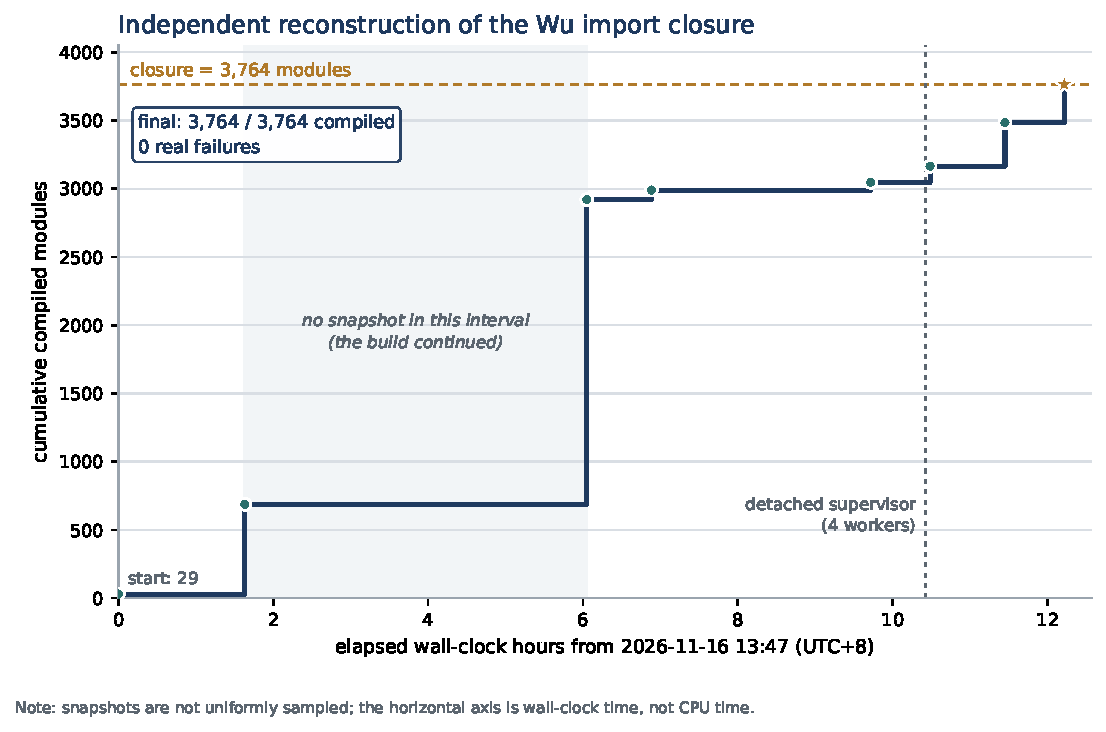
\includegraphics[width=\textwidth]{figures/fig2_progress.pdf}
\caption{Cumulative compilation progress of the Wu import closure. The horizontal axis is wall-clock time, not CPU time; snapshots were not uniformly sampled, so a flat stretch does not mean the build stopped. Final: 3,764/3,764, zero real failures.}
\label{fig:progress}
\end{figure}

The endpoint probe prints six lines, all of the form
\begin{center}
\texttt{depends on axioms: [propext, Classical.choice, Quot.sound]}.
\end{center}
{\raggedright
The six declarations are \texttt{WuLegacyLiteralAcceptance}, \texttt{WuPaper.ClassicalSlots.one8938}, \texttt{WuLiteralAcceptance}, \texttt{WuLiveShapeCheck}, \texttt{WuPaper.ClassicalSlots.one894} and \texttt{WuPaper.ClassicalSlots.classical\_lower}. In particular \texttt{WuLiteralAcceptance} proves a hand-written literal type directly from \texttt{one8938}, and \texttt{WuLiveShapeCheck} proves \texttt{Goldbach.OnePlusOne8938Shape} from the same endpoint, showing that the endpoint's literal type equals the shape definition. The endpoint's own compilation log also prints the three standard axioms for \texttt{one8938}, \texttt{one894} and \texttt{classical\_lower}.
\par}

\subsection{What it proves and what it does not}
\label{sec:wu-scope}

\textbf{What it proves:} under fixed sources, fixed dependencies and a fixed toolchain, all 3,764 import-closure modules were compiled at least once by this pipeline with no real failures; source hashes match the manifest; no forbidden tokens; the endpoint declarations pass the kernel with axiom sets exactly the three standard axioms; and the endpoint module passes \texttt{leanchecker} replay. In one sentence: \emph{this endpoint closure was independently rebuilt in this workspace and passed artifact-level kernel checks.}

\textbf{What it does not prove:}
\begin{enumerate}
\item \textbf{It is not a clean-room rebuild.} \texttt{.ok} markers are reused across sessions; the last segment compiled 617 modules on top of 3,147 existing artifacts. Every module was compiled at least once by this pipeline, but not ``from an emptied \texttt{lib} in one run''. It therefore cannot exclude the extreme case of early artifacts disagreeing with current sources; matching source hashes and per-module logs reduce that risk but do not eliminate it.
\item \textbf{It does not replay 3,764 modules.} \texttt{leanchecker} replays only the new declarations of \texttt{WR2ClassicalCertificate}; it does not replay imported modules and is not a second independent kernel. The accurate sentence is ``the endpoint module passed kernel replay'', not ``the whole closure passed independent kernel replay''.
\item \textbf{It does not build the full 4,151-module scope.} Only the 3,764-module import closure was built locally; the upstream figure of 3,500 compilation receipts plus 651 unchanged dependencies is upstream's accounting, not an independent verification here.
\item \textbf{It does not verify the paper's prose.} The kernel checks the Lean sources under \texttt{src/}; the mathematical argument in the paper explaining why these slots hold lies outside the kernel check, and there is no machine proof that the formal statements agree line by line with the paper's semantics. What can be said is ``the formal endpoint passes the checks'', not ``Wu's paper is verified''.
\item \textbf{It does not change the 12-task ledger.} All 12 tasks in upstream's \texttt{mathematical-status.json} remain \texttt{global\_complete: false}; this build does not change that ledger. The tension between the top-level boolean and the task ledger is discussed next.
\end{enumerate}

\subsection{Scope ledgers and textual tension}
\label{sec:wu-tension}

Upstream's acceptance material contains two tensions that must be noted when citing it.

{\raggedright
First, \texttt{mathematical-status.json} states at the top level \texttt{global\_theorem\_proved: true}, \texttt{global\_wu1894\_theorem\_complete: true} and \texttt{final\_acceptance.status: pass}, while all 12 entries of \texttt{tasks[]} in the same file are \texttt{global\_complete: false}. If the 12 tasks are the ledger of the Wu04/Wu08 source-route recovery, and the final endpoint instead follows the \texttt{WR2Classical*} certificate route, the two can coexist; but the file contains no sentence explaining that switch. If the 12 tasks are treated as mandatory steps towards the endpoint, the true top level directly contradicts the false tasks. We do not interpret the tension for upstream; we report it and recommend that citations say which ledger is meant instead of quoting only the top-level boolean.
\par}

{\raggedright
Second, \texttt{completion-audit.json} is marked \texttt{reviewed\_at\_utc: 2026-10-24}, its scope reaches only $1+1.894$, and it states explicitly ``No separate literal acceptance of 1.8938 is claimed.''; yet \texttt{docs/VERIFICATION.md} and the research README from after 26 October already describe $1.8938$ as accepted. These are different points in time: the 24 October audit cannot be treated as current, and the 26 October README cannot be used to infer that the audit was updated. Our independent rebuild took place on 17 November 2026 and is post-seal supplementary evidence in \texttt{gap-v0.1.2}, which it does not modify; this version, \texttt{gap-v0.1.3}, binds it into the sealed manifest (79 files), while the older version remains unchanged and no new conclusions are written back into the earlier snapshot.
\par}

These tensions do not affect the fact that ``3,764 closure modules were compiled locally'', but they do affect the interpretation of ``what upstream acceptance actually covers''. Writing them out is part of closed-loop verification: an audit that reports only \texttt{PASS} and not the ledger tension remains incomplete.

\subsection{Verdict}
\label{sec:wu-verdict}

The verdict on ``the 3,764-module import closure of the Wu endpoint is independently rebuilt locally and passes artifact-level kernel checks'' is \textbf{artifact-verified (A2)}, with scope: this workspace, fixed toolchain, the 3,764-module import closure, not clean-room, endpoint-module-level replay. The verdict on ``Wu's paper is mathematically verified'' is \textbf{unresolved}; on ``the Goldbach conjecture is proved'' it is \textbf{refuted} (for the material audited here, no unconditional theorem concludes $\BG$); and on ``all 4,151 modules are built'' it is \textbf{unresolved}, because we did not do it.

\section{Synthesis}
\label{sec:synthesis}

\subsection{Claim matrix}
\label{sec:matrix}

Table~\ref{tab:matrix} collects the main claims, methods, evidence levels, verdicts and residual risks. It is the paper in miniature: every yes/no carries a scope, and every scope carries an evidence level.

\begin{table}[htbp]
\centering
\footnotesize
\caption{Evidence matrix of the main claims}
\label{tab:matrix}
\begin{tabularx}{\textwidth}{@{}c
>{\raggedright\arraybackslash}p{0.25\textwidth}
>{\raggedright\arraybackslash}p{0.10\textwidth}
>{\raggedright\arraybackslash}p{0.09\textwidth}
>{\raggedright\arraybackslash}p{0.16\textwidth}
>{\raggedright\arraybackslash}X@{}}
\toprule
ID & Claim & Method & Level & Verdict & Residual / scope\\
\midrule
C0 & The preprint proves the Goldbach conjecture & S1--S3 & B+C+A1 & refuted & v1 only; not a refutation of the authors' other work\\
C1 & Under the literal $\mathcal O$, Theorem~1.1 implies $1+1$ & S3 & A1 & supported & formal statement only\\
C2 & Line 180 lists the current case $G(2n)$ in the induction hypothesis & S1 & B & supported & circularity is this item only; $G(2n-2)>0$ analysed separately\\
C3 & $1+1\Rightarrow$ Chen/LL/Wu & S3 & A1 & supported & formal statement only\\
C4 & The three endpoint predicates are strictly wider & S3 & A1 & supported & representation level, not independence\\
C5 & Endpoint $\Rightarrow1+1$ & --- & --- & unresolved & no known derivation\\
C6 & Local rebuild of the Wu endpoint closure & S4 & A2 & artifact-verified & 3,764; not clean-room\\
C7 & The Wu paper's prose is correct & --- & --- & unresolved & not checked\\
C8 & All 4,151 modules built & --- & --- & unresolved & not done here\\
C9 & Finite verification to $4\times10^{18}$ & S2 & C & supported & finite range\\
\bottomrule
\end{tabularx}
\end{table}

The matrix is read vertically: C0's refutation does not weaken C1's support, and C6's artifact pass does not resolve C7's unresolved status. Each row answers only its own question. It is also read horizontally: the stronger a claim, the more evidence levels it needs; but evidence levels cannot be borrowed across rows.

\subsection{What the loop actually closes}
\label{sec:what-closed}

The three cases close different loops:

\begin{itemize}
\item \textbf{Case one closes the text--formal loop.} The textual audit finds the $\mathcal O$ definition and the line-180 assumption; the formalization fixes ``Theorem~1.1 implies $1+1$'' as A1; the text comparison fixes ``circularity'' as B. The two support each other but do not replace each other.
\item \textbf{Case two closes the definition--direction loop.} Endpoint definitions are transcribed from upstream sources; eight theorems fix the direction; the live-endpoint check confirms the shapes are not hand-copied. The output is not new mathematics but a replayable directional interface.
\item \textbf{Case three closes the source--artifact loop.} Source hashes, build, lexical audit, endpoint probes and \texttt{leanchecker} form one chain, each link with failure semantics. The output is a scope-limited A2, not a mathematical theorem.
\end{itemize}

All three share one negative conclusion: \emph{Goldbach remains open}. Their value is not in repeating it but in separating ``why it is still open'', ``which weak results hold'', ``which artifacts pass'' and ``which claims are refuted''. A report that says only ``Goldbach is unproved'' cannot stop the next ``elementary proof'' from being reported as a breakthrough; a report with a claim matrix at least lets the reader see which claim fails at which level, and whether the failure is checkable.

\subsection{The limits of the loop}
\label{sec:limits-closed}

``Closed loop'' is not ``complete''. This loop has at least three cracks.

First, the \textbf{semantic crack}. Whether a formal statement is faithful to the paper's intent still depends on human transcription and textual argument. We can write the transcription out item by item, cite key definitions to line numbers, and compute the consequences of both readings; we cannot machine-prove that ``the natural-language meaning of line 111 is equation~\eqref{eq:papertheorem}''. This is a general limit of formalization, not one specific to this paper.

Second, the \textbf{independence crack}. We have neither a second independent kernel nor a clean-room rebuild. \texttt{leanchecker} is a module-level replay by the same kernel; \texttt{.ok} reuse means early artifacts were not wiped and redone. Source hashes and per-module logs reduce the risk but cannot upgrade A2 to ``fully independent''. A genuine clean-room run would unpack the sources in an empty directory, fetch dependencies afresh, build in one pass, and be reviewed by a third party; that is future work.

Third, the \textbf{externality crack}. Our audit is single-team, single-environment, single-toolchain. There is no peer review, no author response, no third-party reproduction. We can write down commands, hashes, logs and scopes so that a third party can reproduce or refute; we cannot write ``we found no counterexample'' as ``no counterexample exists''.

\subsection{Reflecting on the originality}
\label{sec:reflexive}

Measured against ``new mathematical theorems'', our original increment is small. Most of the eight main theorems are definitional unfoldings and elementary exponent comparisons; the reconstruction of 3,764 modules copies/confirms an upstream artifact; the refutation of the preprint is an audit of specific text, not new number theory. The project's internal originality audit gives the tiered scorecard: copy/reconstruct 2, audit/correct 2, formalize known facts 9, new structural theorems 5, new mathematical theorems 0, new methods 0; about 415 new physical lines, 14 theorems and 5 definitions locally, against roughly 621,451 physical lines in the Wu closure reviewed, a ratio of about $1:1{,}500$. These numbers should be read as a diagnosis of the type of work, not as an honour for output.

Does the methodological contribution count as a ``new method''? It borrows existing ideas from formalization, reproducible research and evidence grading, and combines them into a protocol for auditing mathematical claims. The combination works in practice, but it is not a wholly new epistemological framework; we prefer to call it ``operational evidence hygiene'' rather than ``a new theory''. Its value lies in reusability: any composite claim facing ``paper + code + formalization + numerics'' can be split with the same table.

This reflection is not self-deprecation but a condition of academic honesty. Verification work usually produces trust infrastructure, whose value grows with use rather than with the number of theorems. If nobody uses these interfaces to prove something new, it stays at the level of ``we checked someone else''. The next step is not to rebuild another thousand modules but to turn the claim matrix into an evidence standard others can cite, and to try it on new claims that have not yet been widely checked.

\subsection{Implications for practice}
\label{sec:implications}

For authors: when submitting a paper that involves computation or formalization, attach an ``evidence statement'' listing item by item which conclusions are kernel-checked, which are finite computations, which are textual arguments, and what the scope and version are. A \texttt{PASS} without a scope carries no information.

For journals and conferences: require formalization papers to provide (i) source hashes and toolchain versions, (ii) a correspondence table between formal statements and the paper's theorems, (iii) the axiom sets and the replay scope, and (iv) a fail-closed statement for finite computations. This will not turn referees into compilers, but it will stop ``formalized'' from being misread as ``the whole paper verified''.

For public communication: state the logical direction of ``$1+2$'', ``$1+1.9$'', ``$1+1.8938$'' and ``$1+1$'' clearly. Weak results are corollaries of $1+1$, not approximate proofs of it; finite verification to $4\times10^{18}$ is empirical evidence, not a proof of an infinite statement; and the existence of a preprint is not peer-review acceptance.

\section{Threats to validity}
\label{sec:threats}

\paragraph{Construct validity.}
We decompose a ``proof claim'' into definitions, quantifiers, circularity and error terms; such a decomposition may miss other kinds of mathematical error (hidden geometric intuition, mis-cited lemmas). We judge only the components we located and do not claim to cover the whole text. The construct validity of formal statements depends especially on human transcription; item-by-item citation, the two readings and the live-endpoint check reduce the risk but cannot remove it.

\paragraph{Internal validity.}
Artifacts of the Wu rebuild may be affected by caching, concurrency and file-system jitter. Measures taken: fixed toolchain, source hashes, per-module logs, retry on failure, and a final completeness gate. But \texttt{.ok} reuse means it is not clean-room; consistency between early artifacts and current sources is supported indirectly by hashes and logs, not by byte-level replay. One \texttt{0xC0000005} observed with 6 workers was attributed to an environment crash because the same module passed with 4 workers; the attribution is reasonable but cannot exclude a very low-probability compiler or hardware fault.

\paragraph{External validity.}
This is a three-case study, not a statistical sample. Whether the framework applies to other areas of mathematics, other proof assistants or other teams requires more cases. We do not write ``works in this project'' as ``works in general''.

\paragraph{Conclusion validity.}
Our negative conclusions concern only the specific line numbers and definitions of arXiv:2611.09007v1; if the authors release v2, they must be re-checked. Our positive conclusions concern only the formal statements listed and the build scope listed; they constitute neither a mathematical verification of the original Chen, Li--Liu or Wu papers nor any advance on the Goldbach conjecture.

\paragraph{Ethics and academic norms.}
We criticise a specific preprint but cite only publicly checkable line numbers and hashes, do not judge the authors' motives, and do not use accusatory vocabulary such as ``fraud''. We leave room for an author response; if the authors point out a misreading, we should re-check by line number and correct. We use upstream open-source code under its Apache-2.0 licence and retain attribution and NOTICE; we do not claim upstream work as our own and claim no priority. Our use of AI is described in the generative-AI statement.

\section{Conclusion}
\label{sec:conclusion}

The binary Goldbach conjecture remains open. This paper does not prove it and does not claim that any weak result suffices to derive it. What it does is split the claims surrounding it into separately checkable parts and show, through three cases, what closed-loop verification looks like in practice.

First, for arXiv:2611.09007v1, under the authors' own $\mathcal O$ the statement of Theorem~1.1 already implies $1+1$; line 180 of the proof lists the current case $G(2n)$ in the induction hypothesis, making the argument circular; the same sentence takes $G(2n-2)>0$ as an input, which under the literal definition already presupposes the positivity required by the conclusion (B) and under the standard reading lacks a basis; and equations (1)--(2) are each off by one in opposite directions for all $3\le x\le6000$. Neither reading supports the proof claim.

Second, eight Lean~4 theorems fix ``$1+1$ implies Chen/Li--Liu/Wu'' and ``the paper's theorem under its own $\mathcal O$ implies $1+1$'' as replayable propositions under the standard axioms; three witnesses show that the endpoint representation predicates are strictly wider, which is neither an independence proof nor a converse.

Third, the 3,764-module import closure of the Wu endpoint was independently rebuilt locally: zero real failures, matching source hashes, six endpoint declarations depending exactly on the three standard axioms, and an endpoint-module \texttt{leanchecker} replay returning 0. The result is artifact-level, not clean-room and scope-limited; it does not verify the prose of Wu's paper and does not change the 12-task ledger.

The methodological conclusion is that \emph{the value of verification lies not in a binary \texttt{PASS} but in a verdict that carries a scope, an evidence level and a residual risk}. An auditable ``unresolved'' carries more information than an unauditable ``pass'', and a precise refutation does more to prevent the next misreading than the sentence ``still open''. Goldbach's conjecture is still waiting for a genuine mathematical proof; until it arrives, we can at least keep ``proof'', ``formalization'', ``numerical verification'' and ``wish'' apart.

\section*{Acknowledgements}
We thank the upstream \texttt{subfish-zhou/goldbach-lean} project for opening the sources and documentation of the Chen, Li--Liu and Wu routes, and the Mathlib and Lean communities for maintaining the toolchain. The audit and formalization were carried out in the local DSH\_MM research environment; collaborators on the earlier sealed package and its evidence archive provided the basis for this study. Errors and judgments remain the authors' responsibility.

\section*{Author contributions, competing interests and funding}
\textbf{Author contributions:} \begin{CJK}{UTF8}{gbsn}宋敏\end{CJK}: textual audit; \begin{CJK}{UTF8}{gbsn}宋瑷成\end{CJK}: research design; \begin{CJK}{UTF8}{gbsn}宋奥菲\end{CJK}: paper writing; \begin{CJK}{UTF8}{gbsn}范钧睿\end{CJK}: formalization; \begin{CJK}{UTF8}{gbsn}胡安\end{CJK} and \begin{CJK}{UTF8}{gbsn}涂源\end{CJK}: build verification. \textbf{Competing interests:} the authors declare none. \textbf{Funding:} this research received no external funding.

\section*{Data and code availability}
{\raggedright
The evidence package includes: the audited preprint's v1 source (SHA-256 \texttt{db1fa071\ldots}); \texttt{Goldbach/Gap.lean}, \texttt{GapChecks.lean}, \texttt{GapLiveChecks.lean}, \texttt{EndpointHierarchy.lean}, \texttt{EndpointHierarchyChecks.lean} and their check logs; the Wu rebuild's \texttt{frontier/wu\_verify/STATUS.json}, \texttt{closure\_audit.json}, \texttt{FINAL\_STATUS.json} and \texttt{AUTO\_VERIFY\_DONE.txt}, together with \texttt{final\_probe.log}, \texttt{final\_leanchecker*.log} and \texttt{WR2ClassicalCertificate.log} under \texttt{frontier/wu\_verify/logs/}; and the figure scripts of this paper. The public repository is \url{https://github.com/songminlhy/goldbach-lean} (tag \texttt{gap-v0.1.3}, commit \texttt{c73fce1}); the evidence package is \cite{evidence} and its DOI is \texttt{10.5281/zenodo.24270135}. The upstream repository is \url{https://github.com/subfish-zhou/goldbach-lean} (Apache-2.0). This version binds the endpoint-hierarchy and Wu status files into the sealed manifest (79 files); the already-sealed \texttt{gap-v0.1.2} (68 files) remains unchanged and is not rewritten in place.
\par}

\section*{Generative AI statement}
Literature organisation, code audit, part of the Lean scripts, the figures and the first draft were produced by a generative-AI instance in the local DSH\_MM environment under goals and acceptance criteria set by the authors; the authors chose the problems, set the evidence thresholds, checked the results and finalized the text. All mathematical assertions are adjudicated by the fixed-version Lean kernel, source hashes and recomputable scripts, not by any model's self-report. AI-generated content is treated as an artifact to be audited rather than an authority, which is itself part of the evidence-grading principle used throughout.

\appendix

\section{Lean declarations and axioms}
\label{app:lean}

\paragraph{Main module.}
\texttt{Goldbach/Gap.lean} contains the following declarations (names taken from the source):

\begin{verbatim}
Goldbach.BinaryGoldbach
Goldbach.ChenTheorem
Goldbach.OnePlusOneNineShape
Goldbach.OnePlusOne8938Shape
Goldbach.goldbachCount
Goldbach.PaperTheorem
Goldbach.binaryGoldbach_implies_chen
Goldbach.binaryGoldbach_implies_onePlusOneNine
Goldbach.binaryGoldbach_implies_onePlusOne8938
Goldbach.chen_second_summand_class_includes_composite
Goldbach.liu_multiplier_class_includes_nontrivial
Goldbach.wu_multiplier_class_includes_nontrivial
Goldbach.goldbachCount_pos_iff
Goldbach.paperTheorem_implies_binaryGoldbach
\end{verbatim}

\paragraph{Live-endpoint check.}
\texttt{Goldbach/GapLiveChecks.lean} contains
\begin{verbatim}
Goldbach.GapLiveChecks.live_one_plus_one_nine_has_shape :
  Goldbach.OnePlusOneNineShape
\end{verbatim}
which is proved directly from the live endpoint \texttt{Goldbach.one\_plus\_one\_nine} and adds no axioms beyond the three standard ones.

\paragraph{Endpoint hierarchy.}
\texttt{Goldbach/EndpointHierarchy.lean} contains five theorems, whose core is
\begin{verbatim}
wu_exponent_implies_liu_exponent
onePlusOne8938Shape_implies_onePlusOneNineShape
onePlusOneNineShape_implies_chen
onePlusOne8938Shape_implies_chen
binaryGoldbach_implies_endpoint_chain
\end{verbatim}
They are not among the eight main theorems but provide the machine check for the hierarchy chain of Section~\ref{sec:hierarchy}.

\section{Reproduction commands}
\label{app:reproduce}

The commands below run on Windows from the repository root \texttt{goldbach/}. The toolchain is fixed by \texttt{lean-toolchain} and \texttt{lake-manifest.json}.

\paragraph{Endpoint directionality and the paper interface.}
\begin{verbatim}
cd frontier
py kernel_verify.py --checks Goldbach\GapChecks.lean ^
    --target Goldbach.Gap --log ..\logs\audit_gap_check_rerun.log
py kernel_verify.py --checks Goldbach\GapLiveChecks.lean ^
    --target Goldbach.GapLiveChecks --log ..\logs\audit_live_shape_check.log
\end{verbatim}
Expected: \texttt{RESULT: PASS}, \texttt{leanchecker} exit code 0, axiom set contained in the three standard axioms.

\paragraph{The Wu closure.}
\begin{verbatim}
cd frontier\wu_verify
py -3 verify_closure.py --root WR2ClassicalCertificate
py -3 final_check.py
\end{verbatim}
Expected: \texttt{closure\_audit.json} has \texttt{status} \texttt{PASS}, and \texttt{FINAL\_STATUS.json} has \texttt{status} \texttt{PASS}. To rebuild, first run
\begin{verbatim}
py -3 build_wu.py --root WR2ClassicalCertificate --workers 4 ^
    --big-kb 120 --big-slots 2
\end{verbatim}
\texttt{.ok} skips finished modules; deleting \texttt{lib} and re-running is a clean-room rebuild, which we did not do.

\paragraph{Numerical audit.}
The numerical audit scripts and results are under \texttt{goldbach/audit/}; we report only their recomputable finite conclusions. The hash of the audited source is in Section~\ref{sec:paper-object}.

\section{Evidence inventory and scope}
\label{app:evidence}

\begin{itemize}
\item \textbf{Audited preprint:} K.~Qazaqzeh, A.~Rawashdeh, \emph{An Elementary Proof of the Binary Goldbach Conjecture}, arXiv:2611.09007v1, 2026-11-06, 9 pages, CC~BY~4.0. Source SHA-256: \texttt{db1fa07154ae7430245d19ac377f6d22f02361608014498fe3449129c3765ffd}.

\item \textbf{Lean toolchain:} Lean~4.33.0-rc1; Mathlib revision \texttt{e4c91783\ldots}; repository tag \texttt{gap-v0.1.3}, commit \texttt{c73fce1}.
\item \textbf{Upstream:} \texttt{subfish-zhou/goldbach-lean}, main at \texttt{9d4c3a4} (2026-10-28), Apache-2.0.
\item \raggedright \textbf{Main-theorem logs:} \texttt{goldbach/logs/audit\_gap\_check\_rerun.log}, \texttt{audit\_live\_shape\_check.log}, \texttt{audit\_chen\_check\_rerun.log}, \texttt{audit\_liliu\_check\_rerun.log}, \texttt{static\_check\_2026-11-15.log}.
\item \textbf{Wu rebuild:} \texttt{frontier/wu\_verify/STATUS.json}, \texttt{closure\_audit.json}, \texttt{FINAL\_STATUS.json}, \texttt{AUTO\_VERIFY\_DONE.txt}, \texttt{logs/final\_probe.log}, \texttt{logs/final\_leanchecker*.log}, \texttt{logs/WR2ClassicalCertificate.log}.
\item \textbf{Scope:} the 3,764-module import closure of Wu; not the full 4,151-module research scope; not the paper's prose; not clean-room.
\end{itemize}

\begin{thebibliography}{99}

\bibitem{chen1973}
J.-R.~Chen,
\emph{On the representation of a large even integer as the sum of a prime and the product of at most two primes},
Scientia Sinica \textbf{16} (1973), 157--176.

\bibitem{chen1978}
J.-R.~Chen,
\emph{On the representation of a large even integer as the sum of a prime and the product of at most two primes. II},
Scientia Sinica \textbf{21} (1978), 421--430.

\bibitem{liliu}
J.~Li and J.~Liu,
\emph{Theorem (1+1.9) on the Goldbach Conjecture},
arXiv:2606.05224 (2026).

\bibitem{upstream}
The goldbach-lean project,
\emph{goldbach-lean: formalized Goldbach routes in Lean~4},
\url{https://github.com/subfish-zhou/goldbach-lean}, Apache-2.0, commit \texttt{9d4c3a4}, 2026.

\bibitem{qazaqzeh}
K.~Qazaqzeh and A.~Rawashdeh,
\emph{An Elementary Proof of the Binary Goldbach Conjecture},
arXiv:2611.09007v1 (2026).

\bibitem{helfgott}
H.~A.~Helfgott,
\emph{The ternary Goldbach conjecture is true},
arXiv:1312.7748 (2013).

\bibitem{oliveira2014}
T.~Oliveira e Silva, S.~Herzog, and S.~Pardi,
\emph{Empirical verification of the even Goldbach conjecture and computation of prime gaps up to $4\cdot10^{18}$},
Mathematics of Computation \textbf{83} (2014), 2033--2060.

\bibitem{llorente2026}
Llorente-Saguer,
\emph{Fail-Closed GPU Verification of the Even Goldbach Conjecture beyond $4\cdot10^{18}$},
Zenodo record 23346739 (2026), preprint.

\bibitem{montgomery-vaughan}
H.~L.~Montgomery and R.~C.~Vaughan,
\emph{Multiplicative Number Theory I: Classical Theory},
Cambridge University Press, 2007.

\bibitem{lean4}
L.~de~Moura and S.~Ullrich,
\emph{The Lean~4 theorem prover and programming language},
Automated Deduction -- CADE 28, LNCS 12699, Springer, 2021, 625--635.

\bibitem{mathlib}
The Mathlib Community,
\emph{The Lean mathematical library},
Proceedings of CPP 2020, ACM, 2020, 367--381.

\bibitem{gonthier2008}
G.~Gonthier,
\emph{Formal proof---the four-color theorem},
Notices of the American Mathematical Society \textbf{55} (2008), 1382--1393.

\bibitem{hales2017}
T.~Hales, M.~Adams, G.~Bauer, et al.,
\emph{A formal proof of the Kepler conjecture},
Forum of Mathematics, Pi \textbf{5} (2017), e2.

\bibitem{scholze2022}
P.~Scholze,
\emph{The liquid tensor experiment},
Experimental Mathematics \textbf{31} (2022), 349--354.

\bibitem{avigad2018}
J.~Avigad,
\emph{The mechanization of mathematics},
Notices of the American Mathematical Society \textbf{65} (2018), 681--690.

\bibitem{geuvers2009}
H.~Geuvers,
\emph{Proof assistants: History, ideas and future},
Sadhana \textbf{34} (2009), 3--25.

\bibitem{peng2011}
R.~D.~Peng,
\emph{Reproducible research in computational science},
Science \textbf{334} (2011), 1226--1227.

\bibitem{donoho2009}
D.~L.~Donoho, A.~Maleki, I.~U.~Rahman, M.~Shahram, and V.~Stodden,
\emph{Reproducible research in computational harmonic analysis},
Computing in Science \& Engineering \textbf{11} (2009), 8--18.

\bibitem{evidence}
DSH\_MM,
\emph{Goldbach gap evidence package: Lean sources, logs, hashes, and timestamped archive},
DOI \texttt{10.5281/zenodo.24270135}, 2026.

\end{thebibliography}

\end{document}
